\section{SReality.cz}
\label{chap:sreality}
Realitní agentura SReality si vytvořila webovou aplikaci, která má ulehčovat uživatelům výběr domu či bytu, ve kterém stráví následující roky svého života. Takové rozhodnutí bývá velmi náročné a proto od sreality.cz očekávam jasné podání informací a hlavně přijatelné uživatelské prostředí. Toto očekávání je znásobené ještě tím, že uživatelé, kteří navštíví danou stránku, mohou být z různých věkových skupin.\\

\subsection{Home page}
\begin{figure}[h]
    \centering
    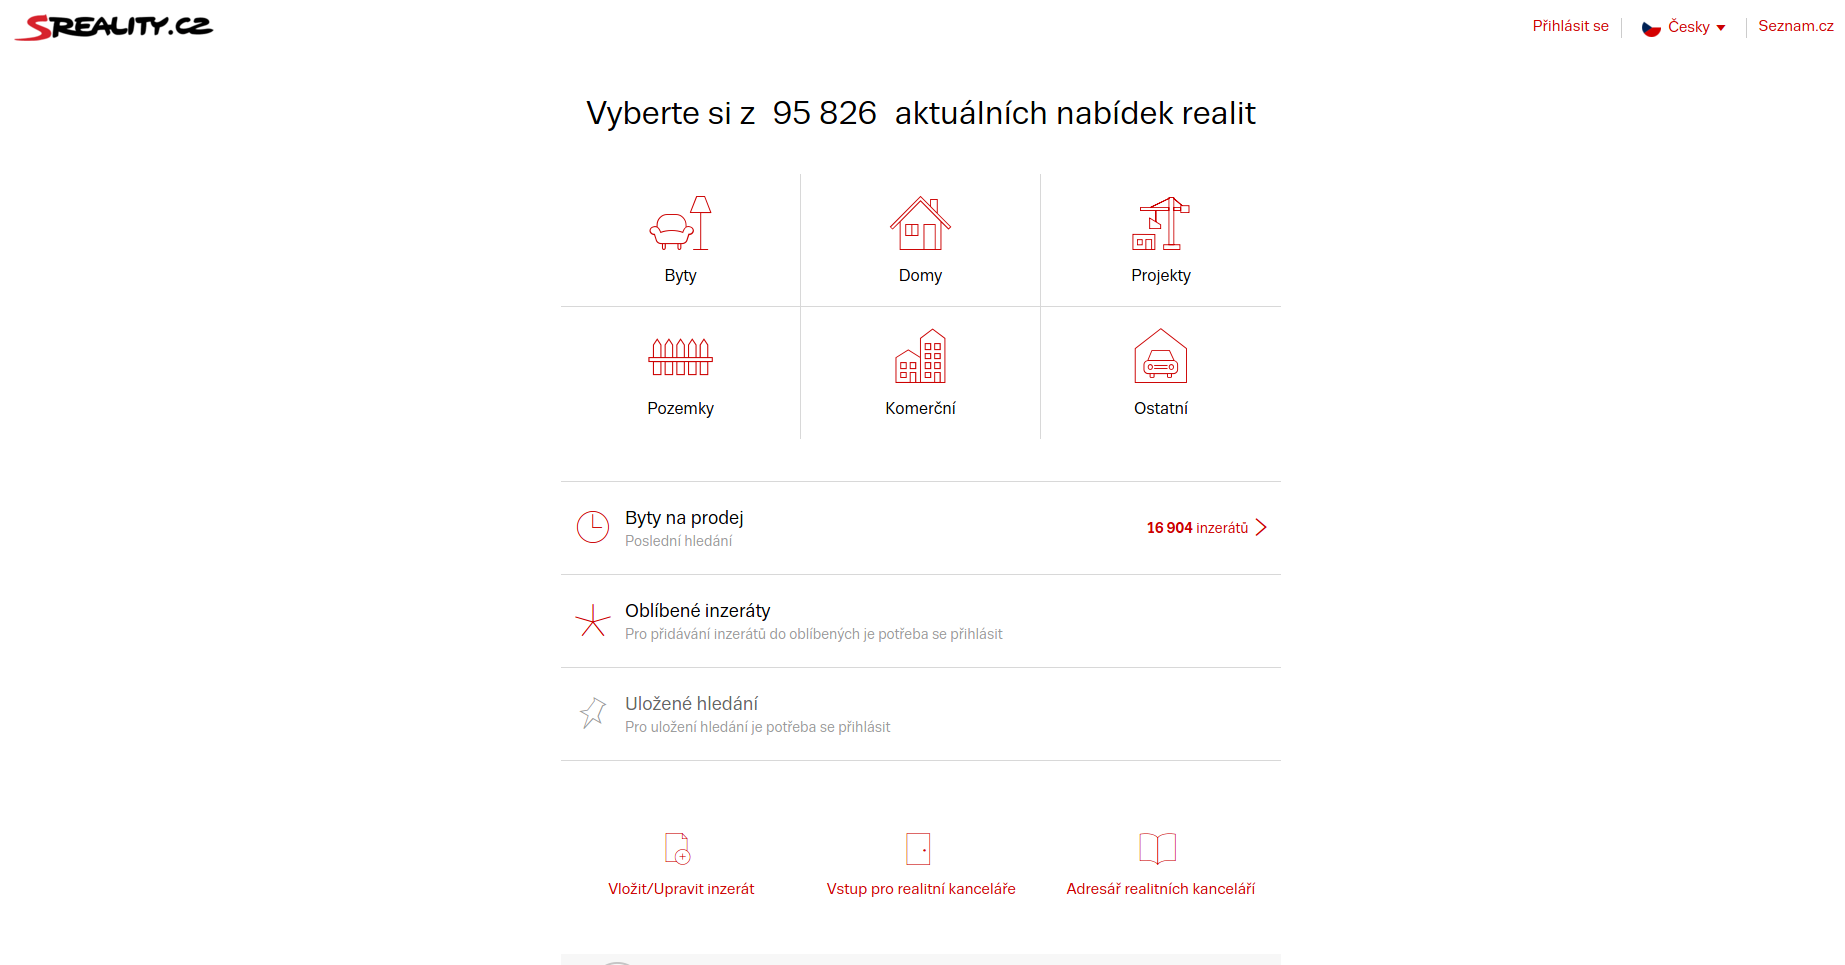
\includegraphics[width=1.0\textwidth]{media/sreality/homepage.png}
    \caption{Hlavní stránka webu sreality.cz}
    \label{fig:sreality:homepage}
\end{figure}
\subsubsection*{Pozitiva}
\begin{itemize}
    \item[+] \textbf{Jednoduchost} -- Bílé prostředí, které obsahuje pouze černé nápisy a červené obrysové nákresy. Velmi jednoduché a přehledné řešení.
    \item[+] \textbf{Poslední a oblíbené vyhedávání} -- Speciální možnosti, které ulehčí hledání uživatelům, kteří již na dané stránce byli a možná si už i nějaké nabídky vybrali.
\end{itemize}
\subsubsection*{Negativa}
\begin{itemize}
    \item[-] \textbf{Nevidím}
\end{itemize}


%%%%%%%%%%%%%%%%%%%%%%%%%%%%%%%%%%%%%%%%%%%%%%%%%%%%%%%%%%%%%%%%%%%%%%%%%%%%%%%%%%%%%%%%%%%%%%%%%%%%%%%%%%%%%%%%%%%%%%%%

\newpage
\subsection{Vyhledávání realit}
\begin{figure}[h]
    \centering
    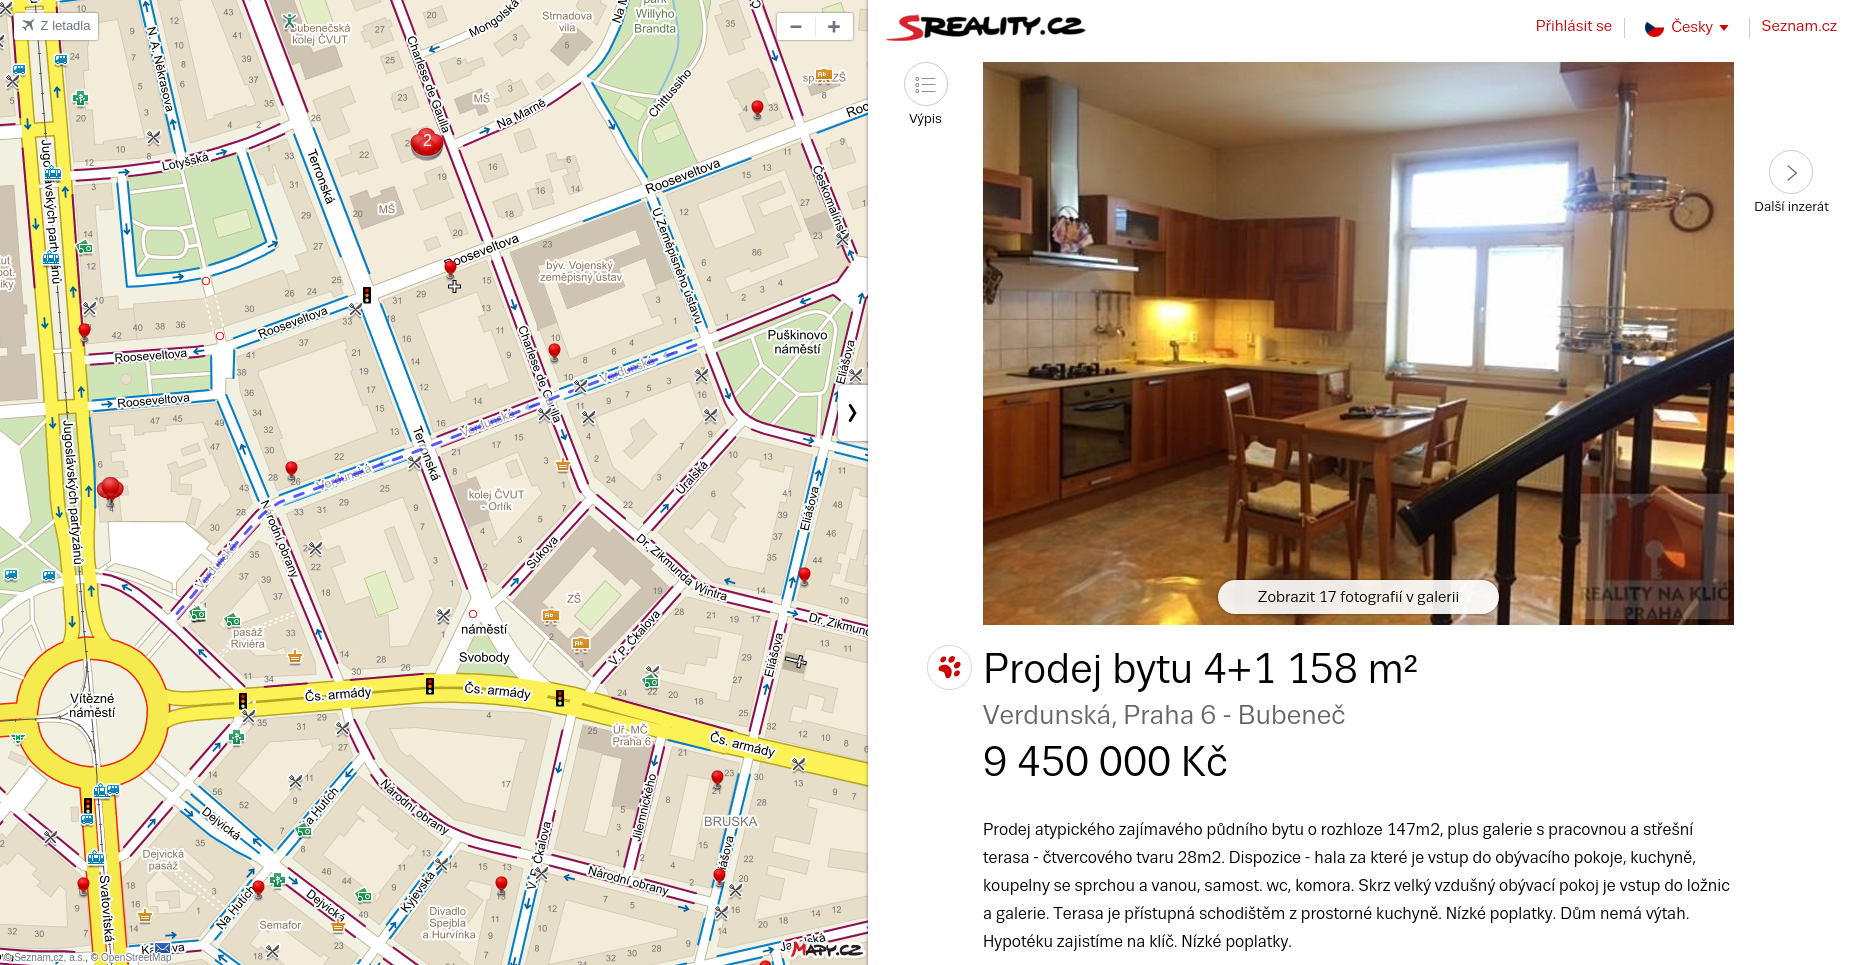
\includegraphics[width=1.0\textwidth]{media/sreality/detail.png}
    \caption{Detail nabídky na webu sreality.cz}
    \label{fig:sreality:detail}
\end{figure}
\begin{figure}[h]
    \centering
    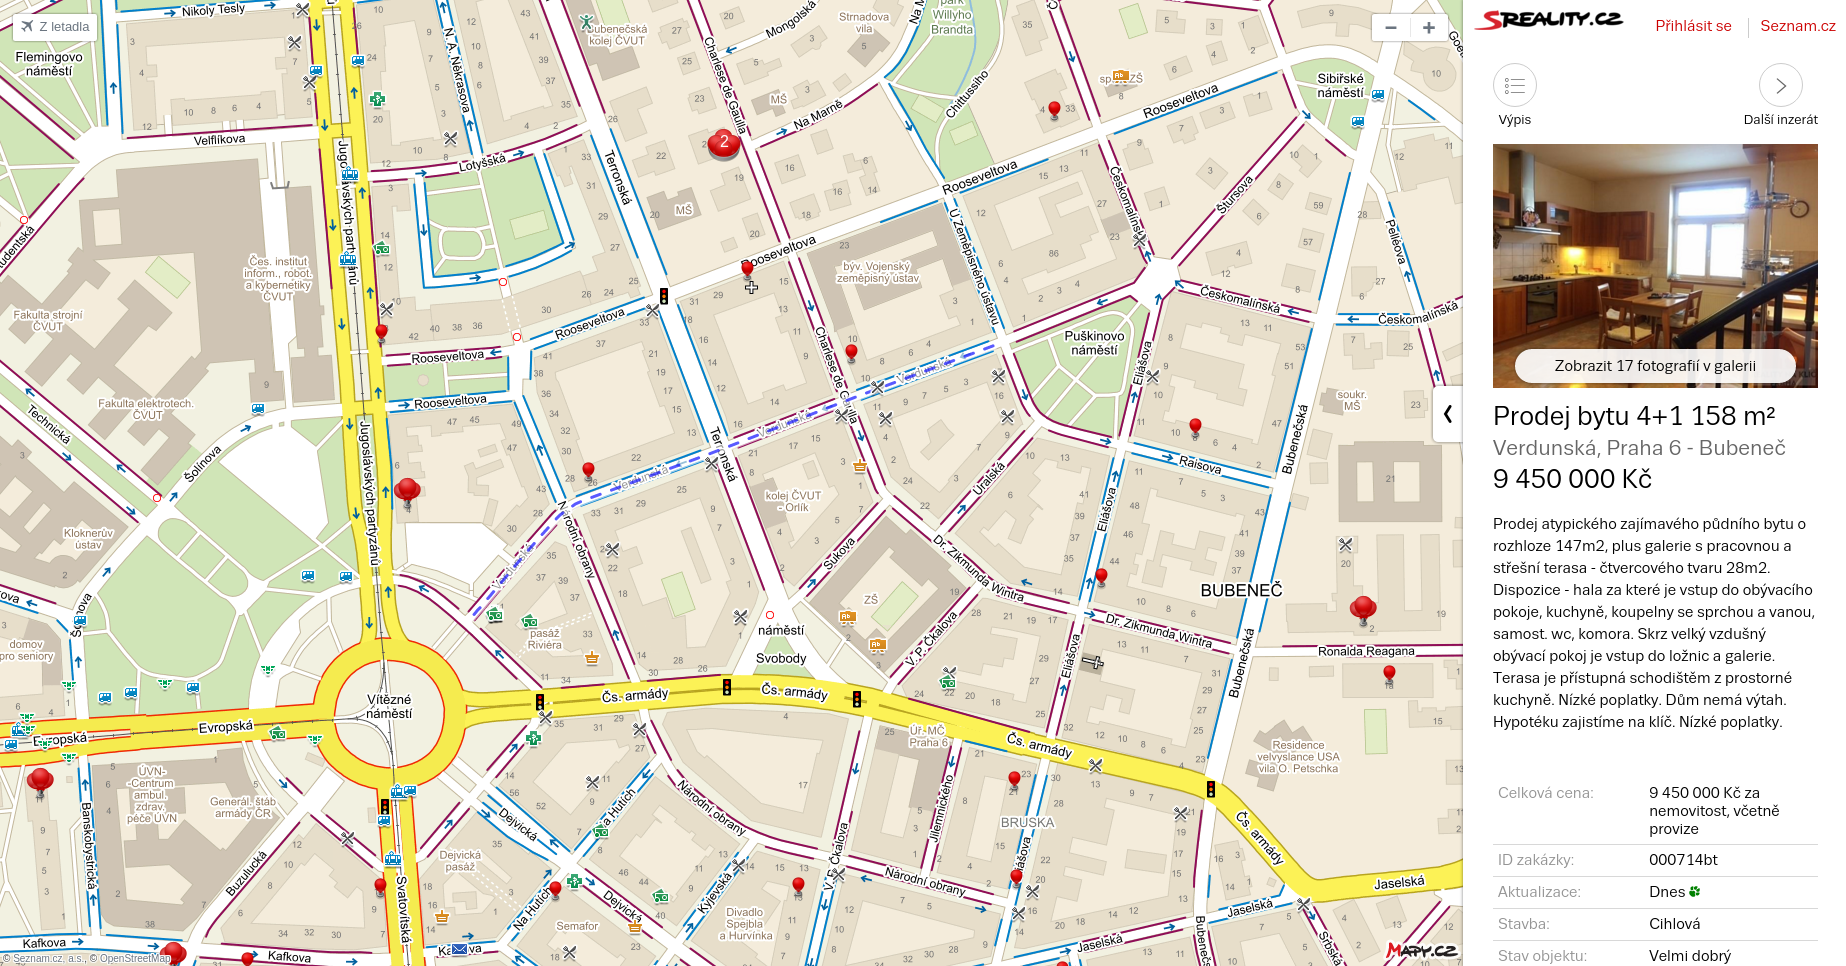
\includegraphics[width=1.0\textwidth]{media/sreality/detail-big-map.png}
    \caption{Detail nabídky na webu sreality.cz - větší mapa}
    \label{fig:sreality:detail-big-map}
\end{figure}
\subsubsection*{Pozitiva}
\begin{itemize}
    \item[+] \textbf{Mapa} -- Krásne propojení seznam map\footnote{mapy.cz a i sreality.cz jsou projekty seznam.cz} a vyhledávání. Navíc je hned vidět jak daleko se nachází zástávka městské hromadné dopravy nebo nejlibžší supermarket a další.
    \item[+] \textbf{Lišta s náhledem nabídky} -- Informativní popis všech vlastností dané nabídky.
    \item[+] \textbf{Zvětšení/zmenšení} -- Uživatel má možnost zvětšit, nebo zmenšit mapu a tím pádem vidět méně či naopak více z obsahu.
\end{itemize}
\subsubsection*{Negativa}
\begin{itemize}
    \item[-] \textbf{Nemožnost čistého náhledu bez mapy} -- Při užším a delším vybírání je možné, že lokalitu mám jako uživatel dobře zmapovanou a tím pádem nepotřebuji vidět mapu (ani v malé formě) na levé straně obrazovky.
\end{itemize}


%%%%%%%%%%%%%%%%%%%%%%%%%%%%%%%%%%%%%%%%%%%%%%%%%%%%%%%%%%%%%%%%%%%%%%%%%%%%%%%%%%%%%%%%%%%%%%%%%%%%%%%%%%%%%%%%%%%%%%%%

\newpage
\subsection{Shrnutí}
Celkově se mi webová aplikace sreality.cz jeví jako velmi dobře řešená.

Nejzajímavějším aspektem SReality.cz se mi jeví přítomnost \textbf{mapy}, která ulehčuje a urychluje výběr. Tuto vlastnost určite chci zakomponovat do své webové aplikace. Forma přepínání mezi mapou a obsahem je řešená \textbf{jednoduše} a uživatelsky přijatelně. Podle mě je však dobré se \textbf{vyvarovat nutnosti vždy zobrazovat mapu} a ponechat tuto funkcionalitu jen jako možnost.

Hodnocení uživalů zde není nijak řešené.